% !TeX encoding = UTF-8
% !TeX spellcheck = en_US

\section{Materials and methods}

The code of this package is separated into three abstract types:
\begin{description}
    \item[SimModel] (2 subtypes) -- Discrete state-space models of the plant, including linear and nonlinear representations. They serve as a wrapper to construct \texttt{StateEstimator} and \texttt{PredictiveController} objects, and also as plant simulators to test the designs.
    \item[StateEstimator] (6 subtypes) -- Closed-loop state observers, both for deterministic and stochastic systems. They produce the full state feedback for the \texttt{PredictiveController}.
    \item[PredictiveController] (3 subtypes) -- Linear and nonlinear MPC are available. An explicit controller based on matrix algebra is also possible for linear description without constraint.
\end{description}

\subsection{Plant models}

The \texttt{SimModel} include two concrete subtypes:
\begin{description}
    \item[LinModel] Linear discrete state-space representations of the plant. Continuous-time models are discretized using zero-order hold for the manipulated inputs, and Tustin's approximation, for the measured disturbances.
    \item[NonLinModel] Nonlinear discrete state-space model of the plant. Continuous-time model are not supported yet but manually calling a differential equation solver can mitigate this.
\end{description}

\subsection{State estimators}

The estimators are all implemented in the predictor form (a.k.a. observer form), that is, they all estimates at each discrete time $k$ the states of the next period $\mathbf{\hat{x}}_k(k+1)$. In comparison, the filter form that estimates $\mathbf{\hat{x}}_k(k)$ is sometimes slightly more accurate. The predictor form comes in handy for control applications since the estimations come after the controller computations, without introducing any additional delays. This is especially true if the observer computations are expensive.

There is six \texttt{StateEstimator}s available at the time of writing, all supporting measured an unmeasured model outputs:
\begin{description}
    \item[SteadyKalmanFilter] Steady-state Kalman filter (a.k.a. asymptotic form). This is the default state estimator for controllers based on \texttt{LinModel} objects.
    \item[KalmanFilter] Time-varying version of the Kalman filter. It can computes the estimation error covariance or be applied in situations where there is no solution to the algebraic Riccati equation.
    \item[Luenberger] Deterministic state observer based on eigenvalue placement.
    \item[UnscentedKalmanFilter] Kalman filter for nonlinear systems relying on the generalized unscented transform. It propagates the mean and covariance of the noise by approximating the state distribution. This is the default state estimator for controllers based on \texttt{NonLinModel} objects.
    \item[ExtendedKalmanFilter] Extended version of the Kalman filter. The Jacobians of nonlinear state-space functions approximate the propagation of the noise, automatically computed by forward mode AD.
    \item[InternalModel] Allows the design of predictive controller based on an internal model structure. The stochastic model of the unmeasured disturbances defaults to integrating white noise for each measured output (customizable). This is equivalent of assuming that the disturbances are constant over the prediction horizon, similarly to dynamic matrix control (DMC).
\end{description}

\subsection{Predictive controllers}

\begin{description}
    \item[LinearMPC] Linear model predictive controller. The default optimizer is OSQP, but other solvers can be used by implementing the \texttt{AbstractOptimizer} interface.
    \item[ExplicitMPC] Explicit linear model predictive controller. The explicit solution is computed offline and stored in a \texttt{ExplicitSolution} object. The \texttt{ExplicitMPC} object is then a wrapper to the \texttt{ExplicitSolution} object.
    \item[NonLinMPC] Nonlinear model predictive controller. The default optimizer is Ipopt, but other solvers can be used by implementing the \texttt{AbstractOptimizer} interface. 
\end{description}

\section{Case studies}

\subsection{CSTR}

\subsubsection{Linear Model}

The example considers a continuously stirred tank reactor (CSTR) with a hot and cold water intakes. The linear model, with the manipulated inputs $\mathbf{u}=\begin{smallmatrix}[
u_c & u_h]'\end{smallmatrix}$ and the liquid level and tempertaure as measured outputs $\mathbf{y}=\begin{smallmatrix}[y_L & y_T]'\end{smallmatrix}$ is constructed with:

\begin{minted}{julia}
using ModelPredictiveControl, ControlSystemsBase
sys = [ tf(1.90, [18, 1]) tf(1.90, [18, 1]);
        tf(-0.74,[8, 1])  tf(0.74, [8, 1]) ]
Ts, uop, yop = 2.0, [20.0, 20.0], [50.0, 30.0]
model = setop!(LinModel(sys, Ts); uop, yop)
\end{minted}
\vspace{-26pt}
\begin{minted}{julia-repl}
Discrete-time linear model with a sample time 
Ts = 2.0 s and:
 2 manipulated inputs u
 2 states x
 2 outputs y
 0 measured disturbances d
\end{minted}

The figure 1 depicts the instrumentation installed on the plant. The \texttt{model} object will be used for two purposes : to construct our controller, and as a plant simulator to test the design.

\subsubsection{Linear Model Predictive Controller}

The objective is to control both the water temperature and level and enforcing a liquid level over 45:

\begin{minted}{julia}
ŷmin, nint_u = [45.0, -Inf], [1, 1]
mpc = setconstraint!(LinMPC(model; nint_u); ŷmin)
\end{minted}
\vspace{-25pt}
\begin{minted}{julia-repl}
LinMPC controller with a sample time Ts = 2.0 s,
OSQP optimizer, SteadyKalmanFilter estimator and:
 15 prediction steps Hp
  2 control steps Hc
  2 manipulated inputs u (2 integrating states)
  4 states x̂
  2 measured outputs ym (0 integrating states)
  0 unmeasured outputs yu
  0 measured disturbances d
\end{minted}

By default, LinMPC controllers use \texttt{OSQP.jl} to solve the problem, soft constraints on output predictions $\mathbf{\hat y}$ to ensure feasibility, and a SteadyKalmanFilter to estimate the plant states\footnote{We could have use an InternalModel structure, to avoid state observer, with \texttt{mpc = LinMPC(InternalModel(model), Hp=15, Hc=2, Mwt=[1, 1], Nwt=[0.1, 0.1])}. It was tested on the example of this page and it gives similar results.}. An attentive reader will also notice that the Kalman filter estimates two additional states compared to the plant model. These are the integrating states for the unmeasured plant disturbances, added at the model inputs here.  Before closing the loop, we initialize the estimates with the actual plant inputs and measurements to ensure a bumpless transfer. Since model simulates our plant here, its output will initialize the states. \texttt{LinModel} objects are callable for this purpose:

\begin{minted}{julia}
u,  y = model.uop,  model() # or equivalently: 
# u,  y = model.uop,  evaloutput(model)
initstate!(mpc, u, y)
\end{minted}

We can then close the loop and test \texttt{mpc} performance on the simulator by imposing step changes on output setpoints $\mathbf{r_y}$ and on a load disturbance $u_l$:

\begin{minted}{julia}
function test_mpc(mpc, model)
    N, ry, ul = 75, [50.0, 30.0], 0.0
    t_data,u_data = Ts*(0:N-1), zeros(model.nu,N)
    y_data,ry_data = zeros(model.ny,N), zeros(model.ny,N)
    for k = 0:N-1
        k == 25  && (ry = [48.0, 35.0])
        k == 50 && (ul = -10.0)
        y = model() # simulated measurements
        u = mpc(ry) # or u = moveinput!(mpc, ry)
        u_data[:,k+1], y_data[:,k+1] = u, y
        ry_data[:,k+1] = ry
        updatestate!(mpc, u, y) # update mpc estimate
        updatestate!(model, u+[0;ul]) # update simulator
    end
    return t_data, u_data, y_data, ry_data
end
t_data, u_data, y_data, ry_data = test_mpc(mpc, model)
\end{minted}

Updating the internal states of \texttt{mpc} prepares the object for the \emph{next} control period. That is why the call is done at the end of the \texttt{for} loop. The same logic applies for \texttt{model}. Lastly, we plot the closed-loop test with \texttt{Plots.jl}:

\begin{minted}{julia}
import Plots, ModelPredictiveControl.SimResult
res = SimResult{LinMPC}(t_data, y_data, ry_data, [;;], 
              u_data, [;;], [;;], [;;], [;;], [;;], mpc)
plot(res)
\end{minted}

\begin{figure}
    \centering
    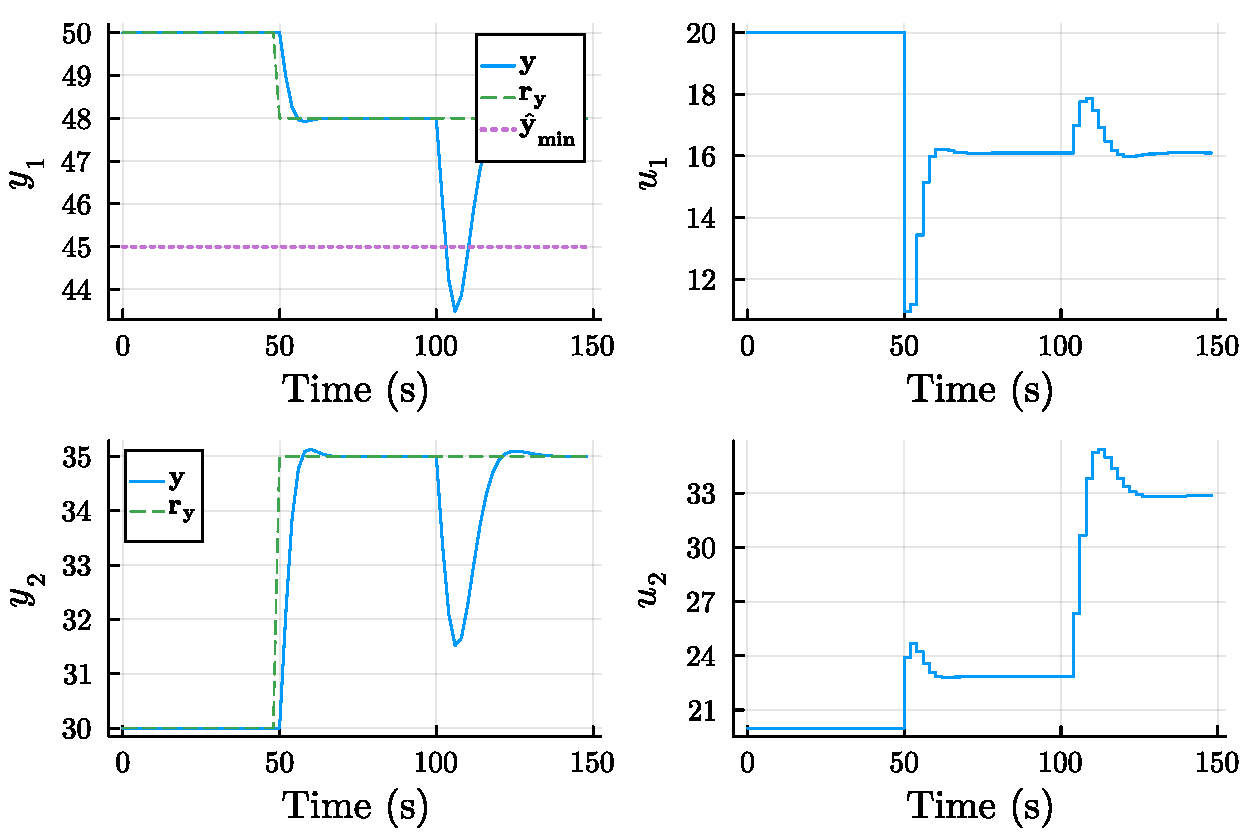
\includegraphics[width=\columnwidth]{fig/plot1_LinMPC.pdf}
    \caption{CSTR closed-loop simulation}
    \label{fig:plot1_LinMPC}
\end{figure}

\cref{fig:plot1_LinMPC} shows that the controller violate the constraints around 110 s. We can improve the performance by adding a feedforward action.

\subsubsection{Adding Feedforward Compensation}

Suppose that the load disturbance $u_l$ of the last section is in fact caused by a separate hot water pipe that discharges into the tank. Measuring this flow rate allows us to incorporate feedforward compensation (FF):

\begin{minted}{julia}
model_ff = LinModel([sys sys[1:2, 2]], Ts; i_d=[3])
model_ff = setop!(model_ff; uop, yop, dop=[20])
\end{minted}

A MPC based on \texttt{model\_ff} and a new function are needed:

\begin{minted}{julia}
mpc_ff = setconstraint!(LinMPC(model_ff; nint_u); ymin)
function test_mpc_ff(mpc_ff, model)
    N, ry, ul = 75, [50.0, 30.0], 0.0
    t_data,u_data = Ts*(0:N-1), zeros(model.nu,N)
    y_data,ry_data = zeros(model.ny,N), zeros(model.ny,N)
    for k = 0:N-1
        k == 25 && (ry = [48.0, 35.0])
        k == 50 && (ul = -10.0)
        y, d = model(), [20 + ul]
        u = mpc_ff(ry, d)
        u_data[:,k+1], y_data[:,k+1] = u, y
        ry_data[:,k+1] = ry
        updatestate!(mpc_ff, u, y, d) # update mpc estimate
        updatestate!(model, u+[0;ul]) # update simulator
    end
    return t_data, u_data, y_data, ry_data
end
\end{minted}

\cref{fig:plot2_LinMPC} shows that the compensation handles the disturbance without violating the constraint.

\begin{figure}
    \centering
    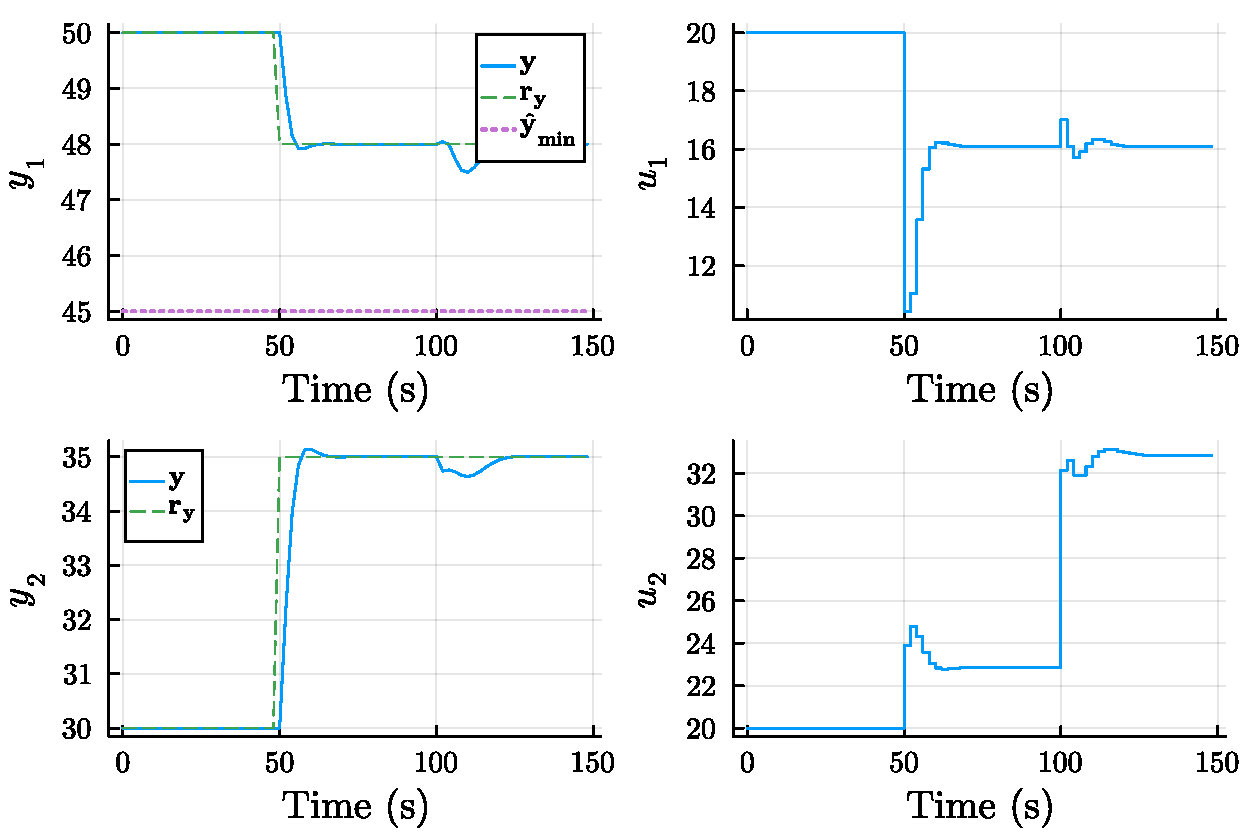
\includegraphics[width=\columnwidth]{fig/plot2_LinMPC.pdf}
    \caption{CSTR closed-loop simulation}
    \label{fig:plot2_LinMPC}
\end{figure}
